\documentclass[10pt]{article}
\usepackage[margin=0.56in]{geometry}
\usepackage{amsmath,amssymb,booktabs,graphicx,microtype,xcolor}

\usepackage[hidelinks]{hyperref}
\setlength{\parindent}{0pt}
\setlength{\parskip}{3pt}
\setlength{\abovedisplayskip}{3pt}
\setlength{\belowdisplayskip}{3pt}
\setlength{\textfloatsep}{5pt}
\renewcommand{\arraystretch}{1.08}

\title{\vspace{-1.15cm}\textbf{Two-Block $4{+}4{\to}8$ Circuit Formation:\\Stationary Theory versus Training}}
\author{}
\date{\vspace{-1.3cm}}

\begin{document}
\maketitle
\vspace{-0.75cm}

\textbf{Result in one sentence.}
Neither protocol forms the $4{+}4{\to}8$ circuit in any of the theory's 34 $H_C$ cells: both fit
the $d8$ target directly in 1k steps, before the parents are accessible, and stay in the
direct phase $H_D$ in all 52 cells that keep it.

\textbf{Experiment.}
The setting of the $d4/d8$ theory: exact eight-bit cube, parents $\chi_L=x_1x_2x_3x_4$,
$\chi_R=x_5x_6x_7x_8$, target $\chi_8=\chi_L\chi_R$ ($\gamma_4=\gamma_8=2$), the bias-free
two-block residual ReLU network of the $d2/d4$ runs ($N=1024$, float64; both readouts read the
final stream $h_2$), and $\lambda_E=\lambda_2=\lambda_p=\lambda_8=\lambda_0$,
$\lambda_1=(\lambda_1/\lambda_2)\lambda_0$ on a $9\times8$ grid ($\lambda_0=10^{-4}$--1,
$\lambda_1/\lambda_2=0.1$--100), seed 0, both protocols.  SGD with momentum 0.9 and rate
$10^{-3}$ for every parameter group, standard initialization (variance $1/$fan-in for every
matrix, readouts included; no $\mu$P), exactly 250k steps, no noise or early stopping.
Parent-warm cells start from $E$, $V_1$, $W_{d4}$ fitted to the parents read from $h_1$ (10k
steps, same optimizer; $R_4=0.097$).

\textbf{Measurements.}  Phase labels, $f_C$, $\varphi_{\rm out}$, $\varphi_{\rm sq}$ and
$f_C^{\rm sq}$ are those of the Langevin report with $\chi_L,\chi_R$ as parents and $\chi_8$ as
target; $R_4=Q_4/Q_1^{(1)}$ (gate $5/32$).  New (Fig.~4): (a) the block-2 share of the parent
amplitude (exact, as $h_0=Ex$ holds only singletons); (b) what block 2's $d8$ producers read: the
$|w_{8,n}a_n|$-weighted share of their pre-activation power on the singletons (direct route
$D_2$), the parents ($C_{44}$), the $\chi_8$ mode already in $h_1$ (a relay of the block-1 route
$D_1$), or degree-2 leakage; (c) $J/\min(F_C,F_D,F_0)$, the final objective over the theory's
minimal free energy ($F_0=3$: zero network).  A cell is \emph{settled} when $J$ changed by
$<1\%$ over the last 50k steps (29 of the 57 non-suppressed cells per protocol).

\begin{center}
\small\setlength{\tabcolsep}{5pt}
\begin{tabular}{@{}lccc@{}}
\toprule
Seed 0, $9\times8$ grid & Parent-warm & Joint & Lower objective \\
\midrule
Phase agreement with theory & 45.8\% & 45.8\% & 45.8\% \\
Gate $H_C\Leftrightarrow R_4>5/32$ (active cells) & 73.1\% & 76.9\% & 76.9\% \\
Mean $|f_C-f_C^{\rm theory}|$ & 0.379 & 0.380 & 0.379 \\
Cells in $H_C$ / $H_D$ / parents only / suppressed (theory: 34/18/0/20) & 0/52/5/15 & 0/52/5/15
 & 0/52/5/15 \\
Cells won (parent-warm / joint) & & & 43/29 \\
$R_4$ when the target is first fitted: median (max) & 0.093 (0.160) & 0.067 (0.140) & \\
$J/\min(F_C,F_D,F_0)$ in settled cells & 0.33--0.93 & 0.33--0.93 & \\
\midrule
Protocols select different phases & \multicolumn{3}{c}{0/72 cells; final $J$ differs by
$\le1.8\%$ (median 0.04\%)} \\
\bottomrule
\end{tabular}
\end{center}

\textbf{Observations.}
(i) \emph{No composition where it is predicted.}  In all 34 theory-$H_C$ cells both protocols
end in $H_D$ with $f_C\le0.05$ (theory 0.66--0.88) and $\varphi_{\rm out}<10^{-5}$ (theory 1);
outside $\lambda_0=0.3$ the $4{+}4{\to}8$ share never exceeds 0.06 along any trajectory.  The
protocols agree in every cell, so the lower-objective row repeats them; pretraining stops at
$R_4=0.097<5/32$ and does not help.
(ii) \emph{The target is fitted before the parents are accessible.}  Every cell that ever fits
$\chi_8$ ($A_8\ge0.5$) does so by the first snapshot (1k steps), at $R_4=0.001$--0.16 (below
$5/32=0.156$ in all but one cell).  $R_4$ crosses the gate only later (1k--230k steps) and only
for $\lambda_1/\lambda_2\le1$, $\lambda_0\ge10^{-3}$ (the 14 parent-warm and 12 joint $H_D$ cells
where the gate disagrees), and the direct routes are not replaced.
(iii) \emph{Block 2 relays or reads raw bits instead of composing} (Fig.~4).  Its $d8$ producers
read the singletons ($\ge97\%$, route $D_2$) for $\lambda_1/\lambda_2\ge5$, and for
$\lambda_1/\lambda_2\le1$ (settled cells) the $\chi_8$ mode that block 1 has already built
(77--99\%): block 2 amplifies $D_1$, a route outside the theory's two families;
$\lambda_1/\lambda_2=2$ mixes the two.  Parents supply $\le9\%$ and degree-2 leakage $\le8\%$ of
these reads, so the $2{+}2{+}2{+}2{\to}8$ route the theory warns about is not used.
(iv) \emph{The parents are partly built in block 2}, since their readouts read $h_2$: 41--64\% of
the joint runs' parent amplitude for $\lambda_1/\lambda_2\le1$ and 78--99\% for
$\lambda_1/\lambda_2\ge10$ (parent-warm 15--58\% and 52--99\%), whereas the theory charges both
parents to block 1 (cost $\propto\lambda_1$).  Block-2 parents cannot feed a $4{+}4{\to}8$ unit.
(v) \emph{Training is cheaper than the closure allows.}  In settled cells
$J=(0.33$--$0.93)\min(F_C,F_D,F_0)$, lowest at large $\lambda_1/\lambda_2$ where the theory pays
$\lambda_1$ for the parents; in the 15 settled theory-$H_C$ cells the $H_D$ networks reach
$J=(0.66$--$0.86)\,F_C$, so the free-energy comparison that places $H_C$ does not bound what
training reaches.  At $\lambda_0=0.1$, $\lambda_1/\lambda_2\ge5$ (theory: suppressed) training
keeps the parents (80--99\% from block 2) and part of the target ($A_8=0.30$--0.46,
$J=2.35$--$2.61<F_0$).  The only compositional block 2, at $(\lambda_0,\lambda_1/\lambda_2)=(0.3,
0.1)$, is also predicted suppressed: $\varphi_{\rm out}=1.00$, $f_C=0.52$, but $A_8=0.22$
($J=2.78$); its neighbour $(0.3,0.3)$ stalls at $J=3.33>F_0$.
(vi) \emph{Weak decay is not stationary.}  Decay alone shrinks the random initial hidden
weights ($\|V\|^2\approx N$) only by $e^{-\eta\lambda t/(1-\beta)}=e^{-0.25}$ at
$\lambda=10^{-4}$ ($e^{-2.5}$ at $10^{-3}$) in 250k steps.  The 28 unsettled cells (all with
$\lambda_0\le10^{-3}$ or $\lambda_1\le10^{-3}$, plus the marginal $(3\times10^{-3},2)$) still lose
1--51\% of $J$ per 50k steps, with $J$ up to $54\times$ the theory's minimum; they include 19 of
the 34 theory-$H_C$ cells and do not test the stationary theory.
(vii) As for $d2/d4$, readout-free and output-weighted shares agree (Fig.~2), and the final
MSE is set by $\lambda_0$, identically for both protocols (Fig.~3).

\textbf{Limits.}  One seed and one optimizer setting.  With the target fitted within 1k steps
and block 2 free to relay $D_1$ or build the parents, this run does not isolate the theory's
two-route competition; that needs parents read from $h_1$, $\chi_8$ and degree-2 leakage
projected out of $h_1$, parents pretrained to $R_4>5/32$ before the target is switched on, and
$\mu$P or a larger rate so that weak-decay cells become stationary.

\begin{figure}[p]
\centering
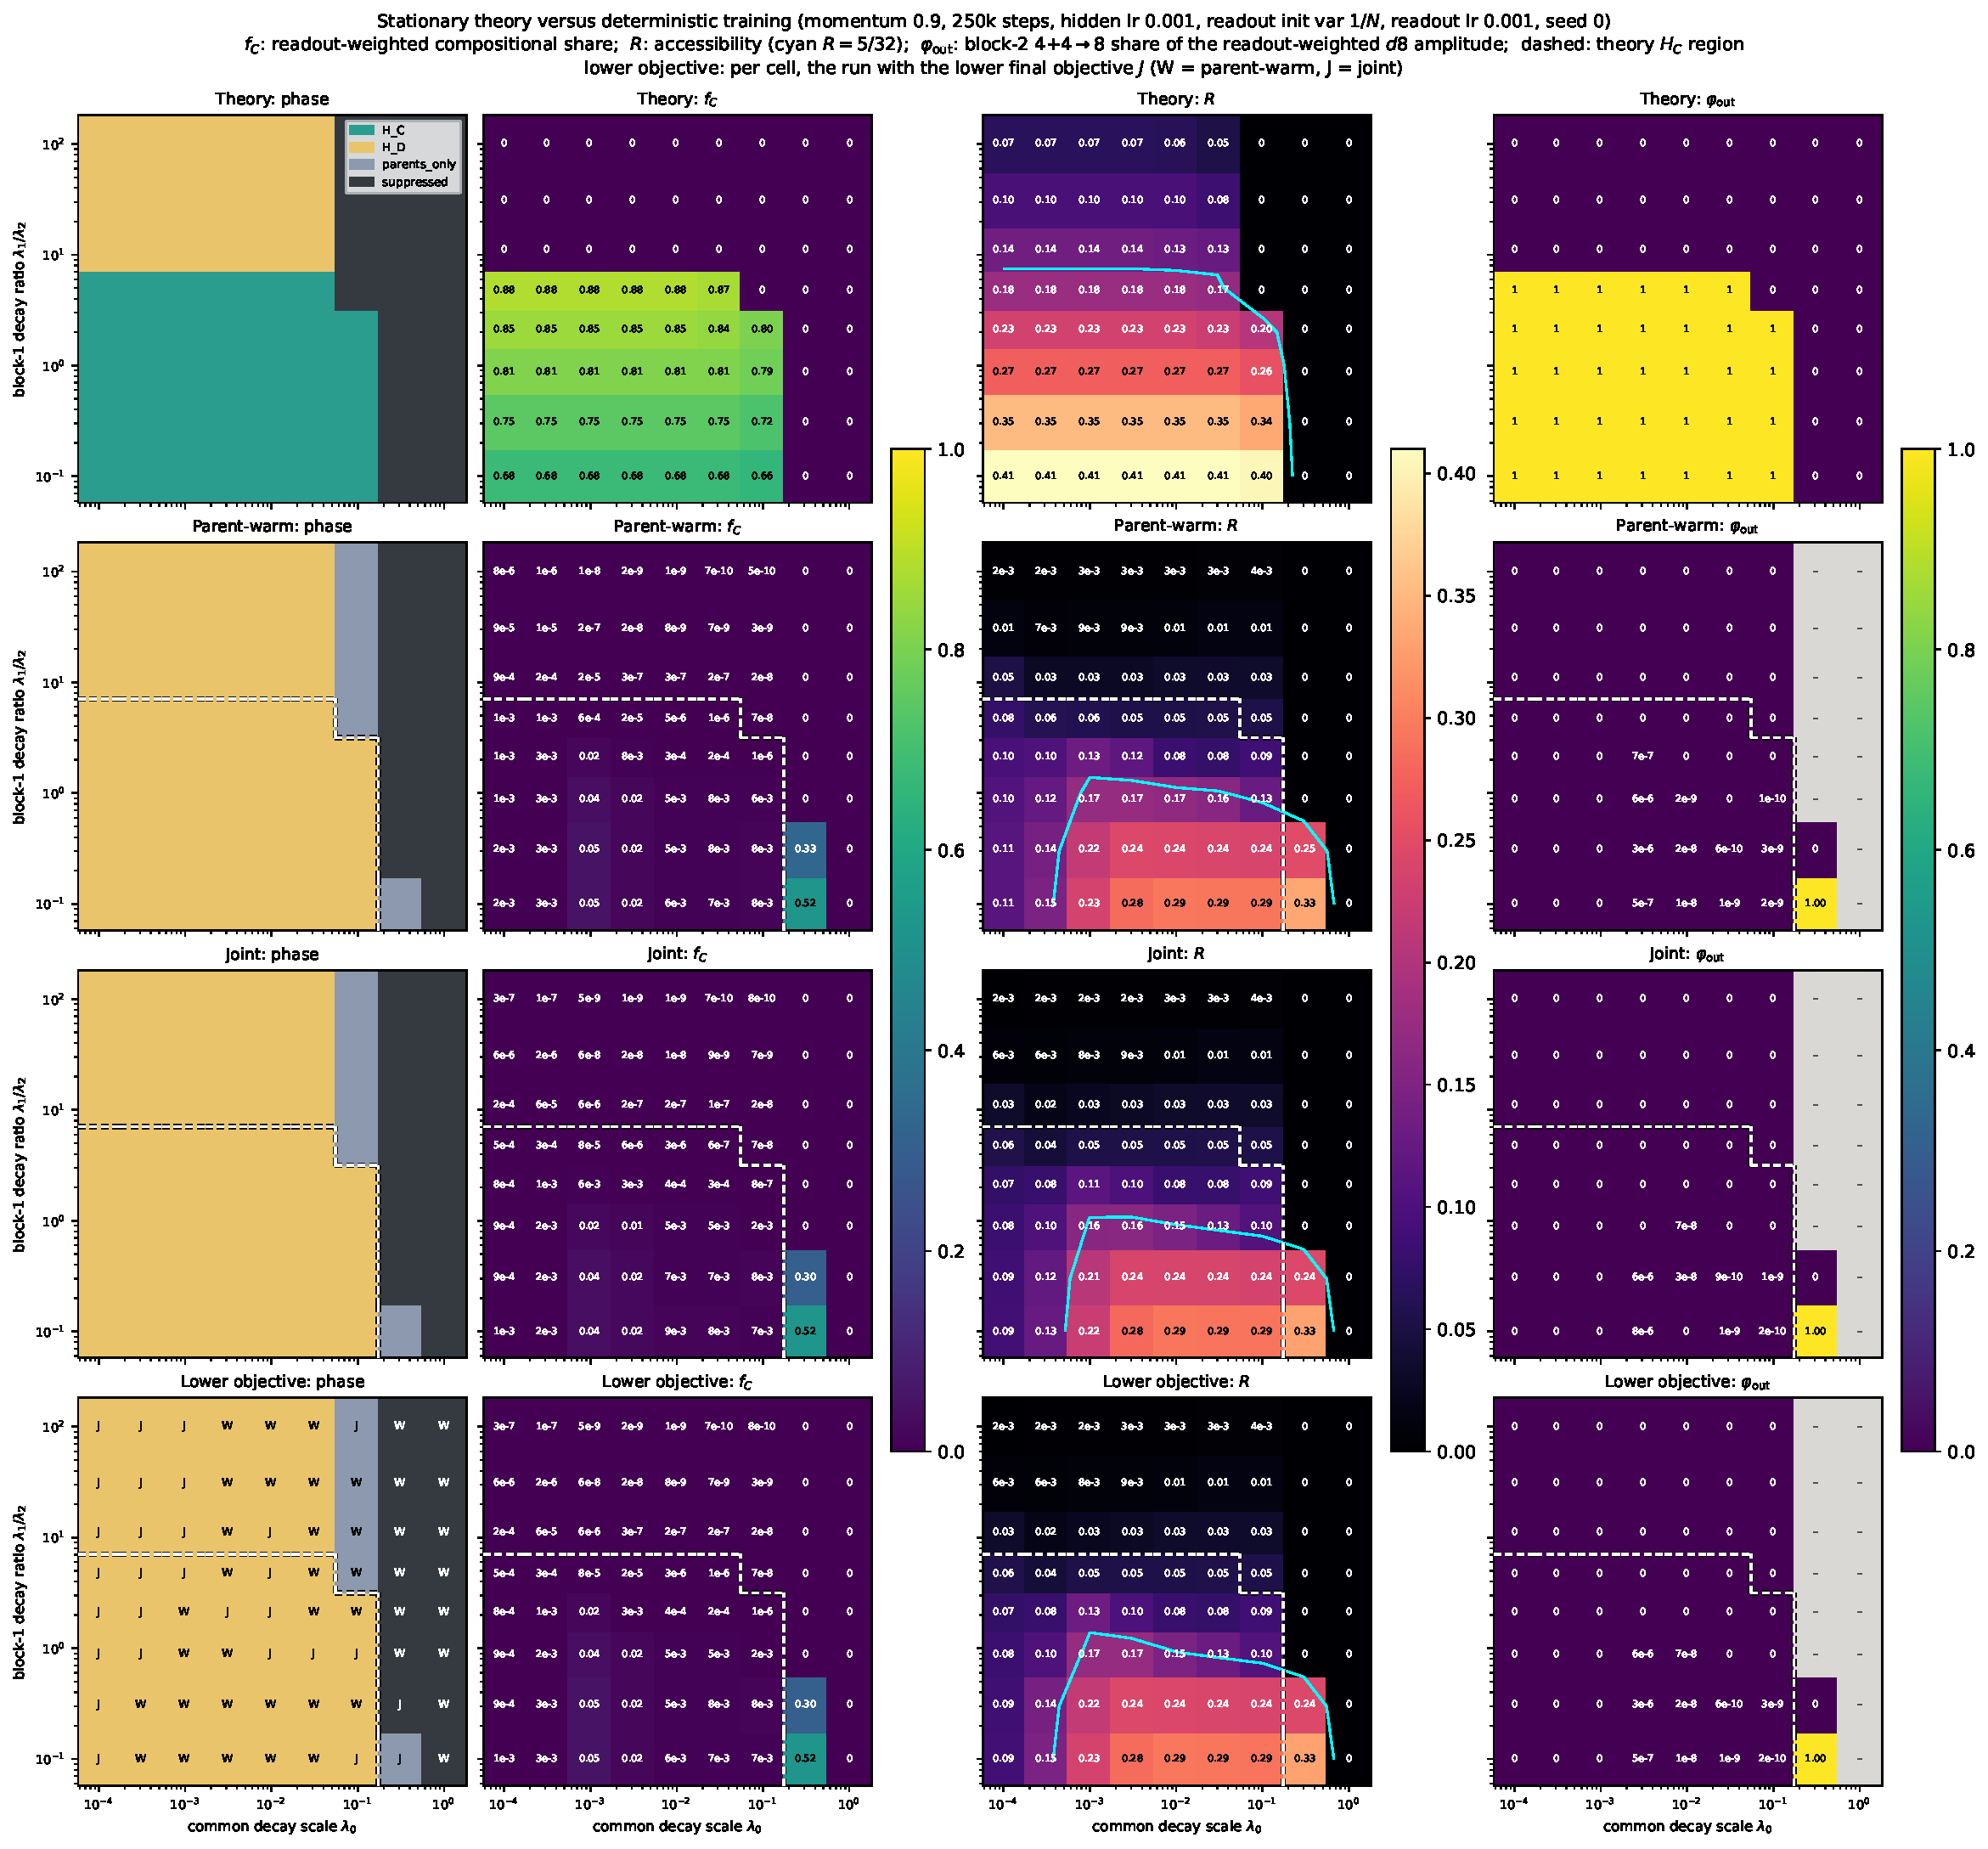
\includegraphics[width=\textwidth]{fig1_theory_vs_annealed.pdf}
\caption{\textbf{Theory, parent-warm, joint, and the lower-objective run per cell (rows, top to
bottom).}  In the bottom row each cell shows whichever of the two runs ended with the lower final
objective $J$ (W = parent-warm, J = joint).  Columns: phase, readout-weighted compositional share
$f_C$, accessibility $R_4$ (cyan: $R_4=5/32$), and the block-2 $4{+}4{\to}8$ share
$\varphi_{\rm out}$ of the readout-weighted $d8$ amplitude.  Dashed: theory $H_C$ region.  Grey:
no target mode produced.}
\end{figure}

\begin{figure}[p]
\centering
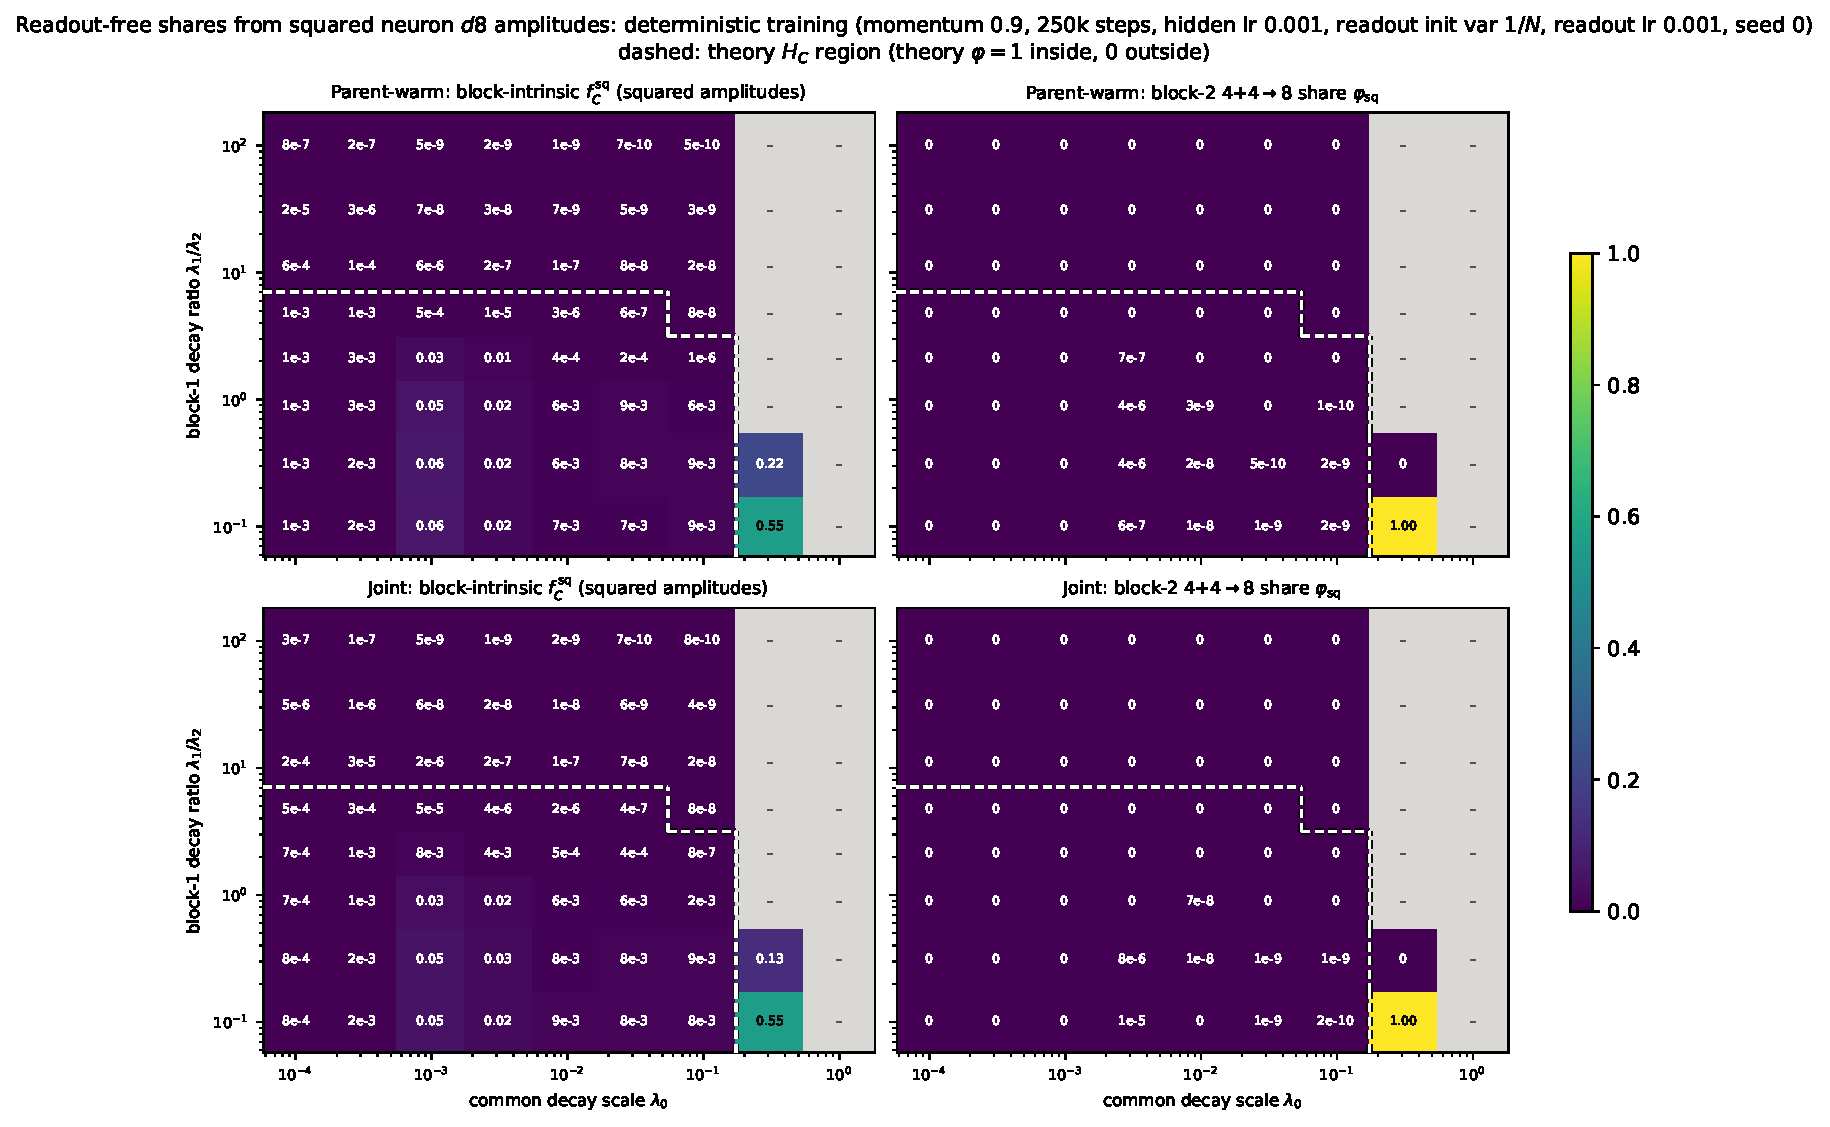
\includegraphics[width=0.78\textwidth]{fig2_block_intrinsic_shares.pdf}
\caption{\textbf{Readout-free shares} from squared neuron $d8$ amplitudes: $f_C^{\rm sq}$ (left)
and $\varphi_{\rm sq}$ (right); compare with columns 2 and 4 of Fig.~1.}
\vspace{6pt}
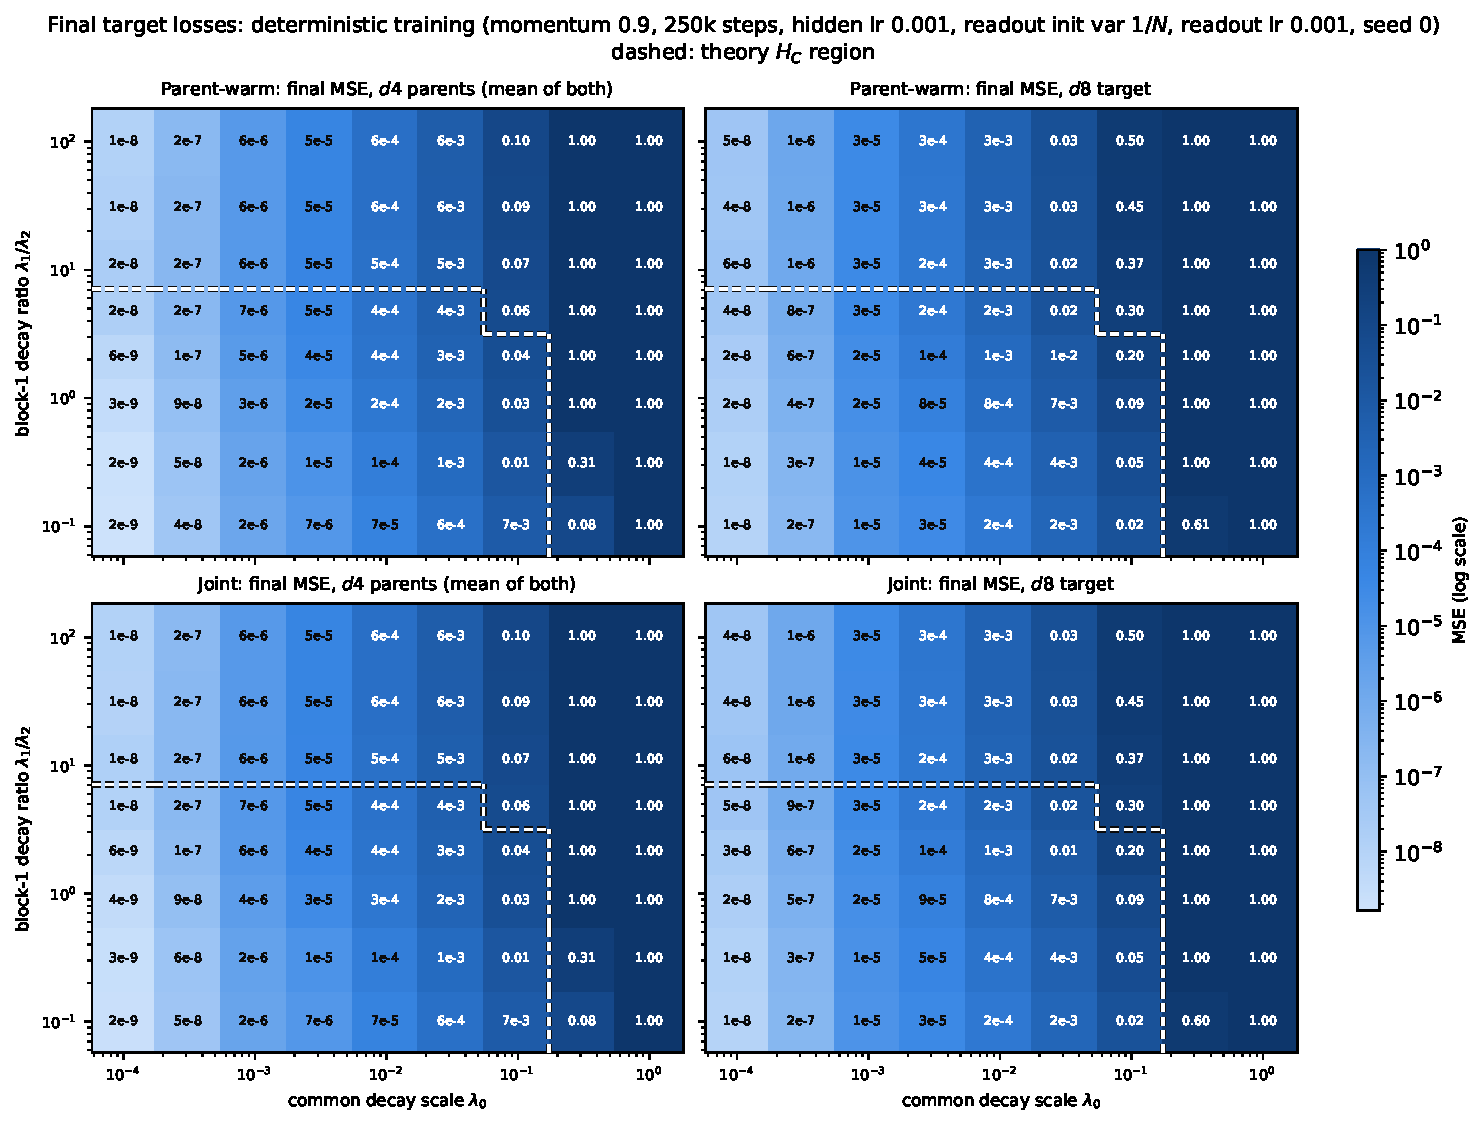
\includegraphics[width=0.78\textwidth]{fig3_final_mse.pdf}
\caption{\textbf{Final losses:} MSE of the two $d4$ parents (mean) and of the $d8$ target, log
scale.}
\end{figure}

\begin{figure}[p]
\centering
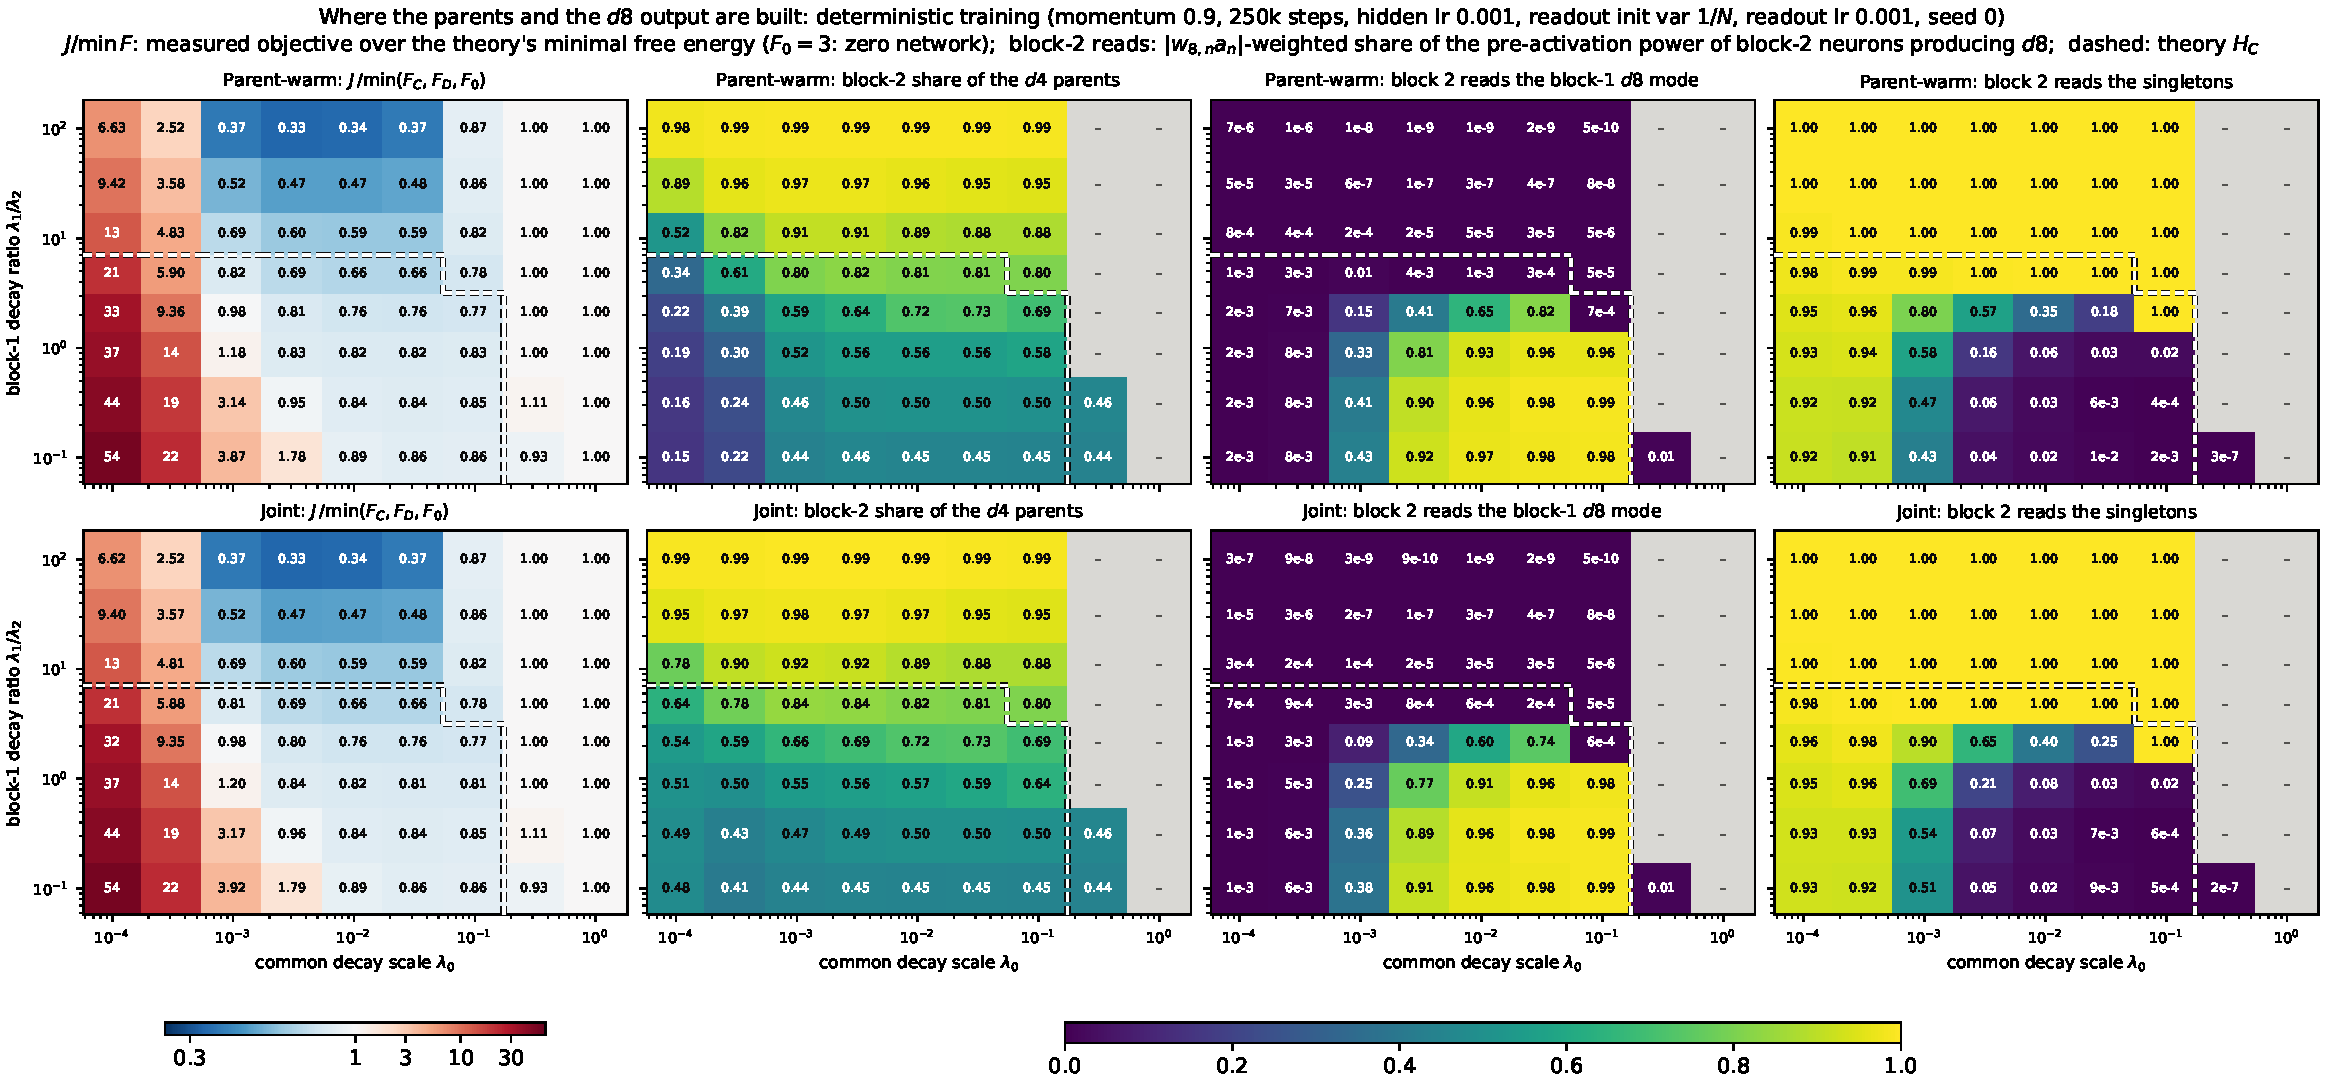
\includegraphics[width=\textwidth]{fig4_route_diagnostics.pdf}
\caption{\textbf{Where the parents and the $d8$ output are built} (rows: parent-warm, joint).
Columns: final objective over the theory's minimal free energy (blue: below it; red: above it,
i.e.\ cells still converging); block-2 share of the readout-weighted parent amplitude; share of
the pre-activation power of block-2 $d8$ producers (weighted by $|w_{8,n}a_n|$) on the $\chi_8$
mode built in block 1 (relay of $D_1$) and on the eight singletons (direct $D_2$).  Grey: block 2
produces no $d8$.  The parent and degree-2 reads ($\le0.09$ outside $\lambda_0=0.3$) are not
shown.}
\end{figure}

\end{document}
